% 第4章 完备市场理论

% 导言

\chapter{完备市场理论与宏观经济学中的均衡}  \label{ch-equilibrium}

目前为止，我们都是从\textbf{计划者}（Social Planner）角度和\textbf{代表性家庭}（同质家庭）的假设下处理最优增长模型。
在计划者问题中，计划者能够直接配置资源而不需要通过市场调节，因此价格并没有显示出现在优化问题中。
那么，计划者问题中的均衡能通过\textbf{市场配置}或者说\textbf{价格机制}实现吗？
即：如果经济是分散的（Decentralized Economy），存在家庭和企业等在市场上的互动，如何定义经济中的均衡，价格在其中起到什么作用？
这一（竞争）均衡产生的配置有什么特征，和计划者问题中的均衡配置有什么关系？
前一章动态规划和递归的框架能在定义均衡中起到什么作用？
代表性家庭的设定又为什么具有合理性？

回答上述问题离不开宏观经济学中的一个重要理论：完备市场（Complete Market）理论。
首先，本章将介绍完备市场理论中两种基础市场结构：\textbf{阿罗-德布鲁市场}和\textbf{序贯市场}；
其次，研究这两种市场下的竞争均衡与计划者问题（帕累托问题）均衡的关系；
同时，我们将指出这两种均衡定义方式的不足，并应用递归的思想定义递归竞争均衡；
再次，应用完备市场理论讨代表性家庭的存在性和资本资产定价问题；
最后，将相关均衡概念应用于一个分散经济下的最优增长模型，通过具体例子深入分析。


% =============== main ch4 ===============


% 4.1 ===== consumption saving =====
% 4.1 =============== Complete Market ===============

\section{完备市场理论基础}  \label{sec-complete-market}


% 4.1.1 ===== 经济环境设定（LS / Edmond / JLao）=====
\subsection{经济环境设定}

经济的时间是离散且无穷的：$t=0,1,\cdots, \infty$。在每一期，都有一个\textbf{随机事件}（Stochastic Event）实现，记为：
$$s_t\in S$$
通常我们将其称之为\textbf{状态}（State）。集合$S$是所有可能发生的事件的集合。记截至$t$时刻，所有实现事件的\textbf{历史}（History）为：
$$s^t = \left(s_0,s_1,\cdots,s_t\right) = \left(s^{t-1},s_t\right)$$
历史$s^t$发生的\textbf{无条件概率}（Unconditional Probability）记为：
$$\pi_t\left(s^t\right)$$
对时刻$t>\tau$，记在$s^{\tau}$实现的条件下，观测到$s^t$实现的\textbf{条件概率}（Conditional Probability）为：
$$\pi_t\left(s^t|s^{\tau}\right)$$
在本章，我们始终假设交易在观测到$s_0$的实现后进行，也就是说：$\pi_0\left(s_0\right)=1$。此外，我们暂时无需假设马尔可夫性。

经济中有$I$个个体（消费者），标记为$i=1,\cdots, I$。个体$i$获得的随机禀赋为$y_t^i\left(s^t\right)$，这一禀赋依赖于实现的事件历史$s^t$，
同时历史$s^t$是公共可观测的。个体$i$选择历史依赖的消费计划（History-Dependent Consumption Plan）：
$$
c^i \equiv \{c_t^i\left(s^t\right)\}_{t=0}^{\infty}
$$
个体（消费者）$i$的偏好为：
\begin{equation}    \label{eq-cm-preference-i}
    \begin{aligned}
        U_i\left(c^i\right) &\equiv \sum_{t=0}^{\infty} \sum_{s^t} \beta^t u_i\left(c_t^i\left(s^t\right)\right) \pi_t\left(s^t\right) \\
            &= \mathbb{E}_0 \sum_{t=0}^{\infty} \beta^t u_i\left(c_t^i\right)
    \end{aligned}
\end{equation}
其中，$\mathbb{E}_0$是基于$s_0$的\textbf{条件期望}。注意这里效用函数除了其自变量的下标不同，
我们同时允许不同个体效用函数本身结构的差异，即效用函数具有下标，即$u_i$，但所有个体的效用$u_i$都符合相关规范化假设，同时假设二次可微性。
此外，假设个体间分享概率$\pi_t\left(s^t\right)$的信息，即可以不使用记号$\pi_t^i$。
经济中的\textbf{可行配置}（Feasibale Allocation）满足资源约束：
\begin{equation}    \label{eq-cm-rc}
    \sum_i c_t^i\left(s^t\right) = \sum_i y_t^i\left(s^t\right), \quad \text { all } t, s^t
\end{equation}


% 4.1.2 ===== 两种交易结构（LS / Edmond / Kruger / PHS）=====
\subsection{两种交易结构}

\textbf{完备市场}是宏观经济学中的重要概念，它与\textbf{不完备市场}的主要区别在于：
经济中存在足够多的如状态依存合约等金融工具（数量覆盖未来所有可能的状态数），
个体通过交易这些工具构建资产组合，进而能够实现任意可行配置，对冲所有个体风险（Idiosyncratic Risk）。
\begin{definition}
    \textbf{状态依存合约}（State-Contingent Claims）是一种支付依赖于未来某个事件（状态）$s^t$是否实现的合约。
    例如如果未来可能发生$\{\text{晴天，下雨}\}$两种状态，消费者可以购买下雨时获得1单位消费品和晴天时获得1单位消费品的合约。
\end{definition}

完备市场可以在如下两种经典的市场结构下实现，我们在此分别介绍。

（1）\textbf{阿罗-德布鲁市场}（Arrow-Debreu Market） 

在Arrow-Debreu结构下，市场只在$t=0$时刻开放，
消费者在市场上交易的是对所有未来时刻$t\geq 1$的消费品的索取权（Complete Set of Contingent Consumption Claims）。
这些索取权是状态依存的（State-Contingent Claims）——依赖于截至$t$时所有可能发生的事件历史$s^t$，也被称为阿罗-德布鲁证券（Arrow-Debreu Security）。
在$t=0$时刻后，签订的合约生效，但没有额外交易再发生，因此这一交易结构也被称为\textbf{零时交易}（Time-Zero Trading）。
在阿罗-德布鲁市场中，由于能交易所有未来时间和可能状态下的消费品索取权（工具足够多），因此阿罗-德布鲁市场天然满足完备市场的定义。
\begin{property}
    阿罗-德布鲁市场天然是完备的。
\end{property}

（2）\textbf{序贯市场}（Sequential Market）

与Arrow-Debreu市场不同，序贯市场中的交易是按期进行的。市场每一期都会重新开放，但是市场上只存在一种
单期状态依存合约（one-period-ahead state-contingent claims）。
在$t$时刻，交易的范围仅针对已实现的历史$s^t$这一条件下所有可能的$s^{t+1}=\left(s^t,s_{t+1}\right)$。
序贯市场也被称为\textbf{阿罗市场}（Arrow Market）或Radner市场，其中的单期状态依存合约被称为\textbf{阿罗证券}（Arrow Securities）。
同样，如果每期都存在足够多的阿罗证券，可以覆盖下期所有可能状态，那么序贯市场也可以达到完备。但是，如果交易工具不足，则序贯交易可能无法达成完备性。
例如我们在后面不完备市场理论中将会看到的，若经济中仅存在单期无风险债券，则市场是不完备的。

\begin{property}
    序贯市场可以达到动态完备（Sequentially Complete）。但如果市场中只存在无风险债券，那么序贯市场是不完备的。
\end{property}

\cref{gr-admarket-tree}和\cref{gr-sqmarket-tree}分别给出了三期情形下一个两状态马尔科夫链在两种市场下的商品空间的例子。
随机事件$s_t\in S=\{0,1\}$。在阿罗-德布鲁市场下（\cref{gr-admarket-tree}），站在$t=0$时刻，$s_0=1$给定，截至$t=3$时刻所有可能的事件历史有8种。
个体在$t=0$时对$t\geq3$时所有8个可能节点下的商品索取权进行交易。
\cref{gr-sqmarket-tree}是在序贯市场下，截至$t=2$时刻实现的一个特定历史，和给定这一实现的历史下，$t=3$时刻的两种可能性。
在$t=2$，个体仅能交易在当前历史$(0,0,1)$下所能达到的$t=3$时节点的商品。

\begin{figure}
    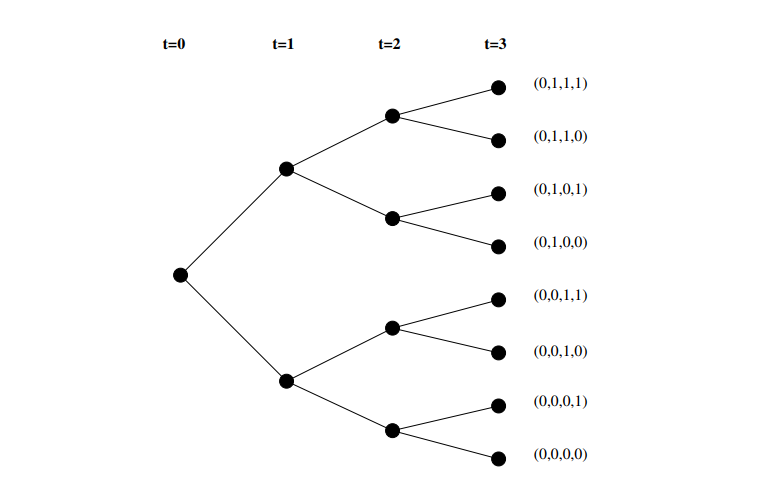
\includegraphics[width=1\textwidth]{figures/part1/ch4/admarket-tree.png}
    \caption{两状态马尔科夫链的阿罗-德布鲁商品空间}
    \label{gr-admarket-tree}
\end{figure}
\begin{figure}
    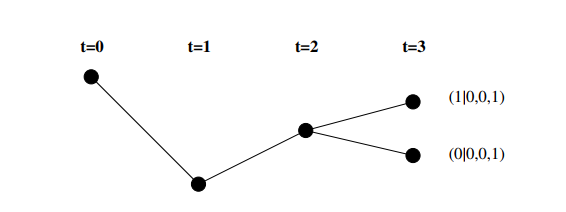
\includegraphics[width=1\textwidth]{figures/part1/ch4/sqmarket-tree.png}
    \caption{两状态马尔科夫链的阿罗-德布鲁商品空间}
    \label{gr-sqmarket-tree}
\end{figure}

两种市场结构对比而言，阿罗-德布鲁市场更近似一个理论基准，而序贯交易相对更贴近于现实市场。
此外，对于上述两种市场结构，我们很自然的会想到如下问题：
\begin{itemize}
    \item \textbf{两种市场中的均衡配置相同吗，与计划者均衡配置有什么关系？}
    \item \textbf{消费者的最优配置是否依赖于历史（History-Dependent）？}
\end{itemize}

我们将证明：两种市场交易结构会带来相同的帕累托最优配置，并且在完备市场下，$t$时刻的最优消费配置仅依赖部分刻画$t=0$时刻财富分布的时不变参数
和$t$时刻经济所实现的总禀赋，不会依赖带来相应总禀赋的历史。


% 4.1.3 ===== 计划者问题（Pareto Problem）=====
\subsection{帕累托问题}

在研究上述两种市场均衡配置的特征前，我们希望先定义一个基准配置用于进行比较，一个自然的想法是帕累托最优。
帕累托最优是指，无法使一个个体变得更好而同时不使其他个体变得更差。如果一个配置是帕累托最优的，我们称其为有效（efficient）。
我们可以通过为计划者解如下\textbf{帕累托问题}（Pareto Problem）找到一个有效配置。

计划者为每个个体$i=1,\cdots,I$选择$c^i \equiv \{c_t^i\left(s^t\right)\}_{t=0}^{\infty}$来最大化如下目标：
\begin{equation}    \label{eq-pareto-maxU}
    W=\sum_{i=1}^I \lambda_i U_i\left(c^i\right)
\end{equation}
其面临的资源约束为：
\begin{equation}    \label{eq-pareto-rc}
    \sum_i c_t^i\left(s^t\right) = \sum_i y_t^i\left(s^t\right) \quad \forall t, s^t
\end{equation}
其中$\lambda_i$是非负的\textbf{帕累托权重}（Pareto Weights）。
如果一个配置能构成一组非负权重下\textbf{上述问题的解}，我们就称这一配置为\textbf{帕累托有效}（Pareto Efficient）。
对这一优化问题，构建拉格朗日函数：
\begin{equation*}
    \begin{aligned}
        \mathcal{L} &= \sum_i \lambda_i \sum_{t=0}^{\infty} \sum_{s^t} \beta^t u_i\left(c_t^i\left(s^t\right)\right) \pi_t\left(s^t\right)
                    + \sum_{t=0}^{\infty} \sum_{s^t} \theta_t\left(s^t\right) \sum_i\left[y_t^i\left(s^t\right)-c_t^i\left(s^t\right)\right] \\
                    &= \sum_{t=0}^{\infty} \sum_{s^t}
                    \left\{\sum_{i=1}^I \lambda_i \beta^t u_i\left(c_t^i\left(s^t\right)\right) \pi_t\left(s^t\right)
                        +\theta_t\left(s^t\right) \sum_{i=1}^I\left[y_t^i\left(s^t\right)-c_t^i\left(s^t\right)\right]\right\} \\
                    &= \sum_i \sum_{t=0}^{\infty} \sum_{s^t}
                    \left\{\lambda_i \beta^t u_i\left(c_t^i\left(s^t\right)\right) \pi_t\left(s^t\right)
                        +\theta_t\left(s^t\right)\left[y_t^i\left(s^t\right)-c_t^i\left(s^t\right)\right]\right\}
    \end{aligned}
\end{equation*}
其中非负的$\theta_t\left(s^t\right)$为第$t$期和历史$s^t$对应约束的拉格朗日乘子。
从这一优化问题的形式上看，计划者实际面临的是一个静态问题（Static Problem）序列，因为问题中并不涉及跨期变量。
具体看，对$c_t^i\left(s^t\right)$求解FOC得：
\begin{equation}    \label{eq-pareto-foc}
    \lambda_i \beta^t u_i^{\prime}\left(c_t^i\left(s^t\right)\right) \pi_t\left(s^t\right)=\theta_t\left(s^t\right) \quad \forall i, t, s^t
\end{equation}
不失一般性，取个体$i$和个体$1$，将他们的FOC结合可得：
\begin{equation}    \label{eq-pareto-r-foc}
    \frac{u_i^{\prime}\left(c_t^i\left(s^t\right)\right)}{u_1^{\prime}\left(c_t^1\left(s^t\right)\right)}=\frac{\lambda_1}{\lambda_i}
        \quad \forall t, s^t
\end{equation}
也即：
\begin{equation}    \label{eq-pareto-ci}
    c_t^i\left(s^t\right)=u_i^{\prime-1}\left(\frac{\lambda_1}{\lambda_i} u_1^{\prime}\left(c_t^1\left(s^t\right)\right)\right)
\end{equation}
这意味着任意个体的消费都可以写为关于个体1的消费$c_t^1\left(s^t\right)$的函数。进一步，将上式代入资源约束\ref{eq-cm-rc}可得：
\begin{equation}    \label{eq-pareto-c1}
    \sum_i u_i^{\prime-1}\left(\frac{\lambda_1}{\lambda_i} u_1^{\prime}\left(c_t^1\left(s^t\right)\right)\right)
        =\sum_i y_t^i\left(s^t\right) \equiv Y_t\left(s^t\right) \quad \forall t, s^t
\end{equation}
注意到，式\ref{eq-pareto-c1}是关于$c_1^t\left(s^t\right)$的单一非线性方程（Single Nonlinear Equation）。
右侧对$i$的求和可以定义为经济的\textbf{总禀赋}，而由于帕累托权重$\{\lambda_i\}_{i=1}^I$是一组给定的参数，因此左侧对$i$求和后也与个体$i$无关，
进而可以从中解出$c_t^1\left(s^t\right)$。

进一步观察式\ref{eq-pareto-c1}可知，给定一组外生参数$\{\lambda_i\}_{i=1}^I$，$c_t^1\left(s^t\right)$\textbf{只依赖当前实现的总禀赋}，
既不依赖时刻$t$，也不依赖特定的能够带来当前总禀赋的历史$s^t$或是在$t$时刻个体禀赋的分布。
同时，式\ref{eq-pareto-ci}将$c_t^i$表为了$c_t^1\left(s^t\right)$的函数，从而可得其余所有个体的消费配置$c_t^i\left(s^t\right)$：
同样是只依赖于所实现的总禀赋的。至此，我们就得到了计划者在参数$\{\lambda_i\}_{i=1}^I$下的一个帕累托有效配置，且均衡解的形式是一个时不变函数：
\begin{equation*}
    c_t^i\left(s^t\right) = f\left(\lambda_i, Y_t ; \boldsymbol{\lambda}\right)
\end{equation*}

\begin{property}
    对于计划者的帕累托问题，一组\textbf{有效配置}具有如下特征：
    \begin{itemize}
        \item 与时间$t$无关，与历史无关（\textit{history-independent or history-free}）：当前的$Y_t$是所有历史的充分统计量；
        \item 与$t$时刻个体禀赋的分布无关（\textit{distribution-free}）：只有求和后的$Y_t$重要。
    \end{itemize}
\end{property}
假设存在两条不同历史路径$s^t$和$\tilde{s}^{\tau}$，但只要$Y_t\left(s^t\right)=Y_{\tau}\left(\tilde{s}^{\tau}\right)$，
就有$c_t^i\left(s^t\right)=c_{\tau}^i\left(\tilde{s}^\tau\right)$。

进一步观察\ref{eq-pareto-r-foc}式，对任意两个个体$(i,j)$成立：
\begin{equation*}
    \frac{u_i^{\prime}\left(c_t^i\left(s^t\right)\right)}{u_j^{\prime}\left(c_t^1\left(s^t\right)\right)}=\frac{\lambda_j}{\lambda_i}
        \quad \forall t, s^t
\end{equation*}
也就是说，\textbf{在任何有效配置中，个体间消费边际效用比在任意时刻、任意历史下都相等}。
背后的经济含义是:计划者通过维持不同个体间消费边际效用比来为所有个体在任意时间和状态下提供\textbf{消费保险（Consumption Insurance）}。
由于计划者问题中除了总的资源约束外不存在其他约束，因此很自然的将这一情形定义为\textbf{完美消费保险}（Perfect Consumption Insurance）或
\textbf{完美风险承担}（Perfect Risk Sharing）。

\begin{definition}  \label{def-perfect-c-insurance}
    \textbf{完美消费保险}（Perfect Consumption Insurance），或称\textbf{完美风险承担}（Perfect Risk Sharing），
    是指一组消费配置$\{c^i=\{c_t^i\left(s^t\right)\}_{t=0}^{\infty}\}_{i=1}^{I}$：
    使不同个体间的消费边际效用比在任意时刻、任意状态下都相同（Constant across any time and states）。
\end{definition}

至此，我们通过求解计划者的帕累托问题，建立了一个基准均衡配置。这一均衡是\textbf{帕累托有效}的，因为计划者不可能使某一个体变好而不使其他人变差。
从计算的角度看：我们通过式\ref{eq-pareto-c1}解出$c_t^1\left(s^t\right)$，
再通过式\ref{eq-pareto-ci}解出其余个体的$c_t^i\left(s^t\right)$。并且由式\ref{eq-pareto-ci}可知：
只有不同个体间帕累托权重的比值是值得关注的。因此，我们可以进行正则化，将权重和定为1：$\sum_{i}\lambda_i = 1$。
由于每个个体的消费配置只是总禀赋的函数，因此其个体消费与总禀赋（总消费）完全相关，并且所占份额与其所分配得的帕累托权重相关。



% 4.2 ===== consumption saving =====
\input{parts/part1/p1c4/p1c4-2-ra-existence.tex}


% 4.3 ===== consumption saving =====
% 4.3 =============== CAPM ===============

\section{资本资产定价（CAPM）}  \label{sec-capm}




% 4.4 ===== consumption saving =====
\input{parts/part1/p1c4/p1c4-4-decentralized-equlibrium.tex}

